\chapter{Introduction}

\section{Introduction}
Fusion techniques are very common in our nature. Animals sense the environment by eyes, ears etc. We, Humans, also have the ability to collect data about the environment model by five body senses. We can enrich the perceived environment model by combining all senses data \cite{Wilfried2002}. Like nature, science also adopt the fusion concept and successfully applied in its many fields. For example, self driving car needs to sense the environment by the sensors and sensor fusion helps to perceive the environment model more correctly. This paper tries to explain the basic concept of Sensor Fusion and also explains some of the applications of this concept.

\section{What is Sensor Fusion?}
The term \emph{Sensor Fusion} means fusing multiple sensor data to make a rich environment model. One sensor data may not cover all the information or in some cases one sensor may produces incomplete information. Fusion of multiple sensors data improves the quality of the data and produce more reliable environment model. According to \cite{Hall:2004:MTM:1204261} the term \emph{multisensor data fusion} defined as,
\theoremstyle{definition}
\begin{definition}{Multisensor data fusion}
is the technology concerned with the combination of how to combine data from multiple (and possible diverse) sensors in order to make inferences about a physical event, activity, or situation.
\end{definition}
On the other hand, the more formal definition of Sensor Fusion is defined in \cite{Wilfried2002} as,
\theoremstyle{definition}
\begin{definition}{Sensor Fusion}
is the combining of sensory data or data derived from sensory data such that the resulting information is in some sense better than would be possible when these sources were used individually.
\end{definition}
There is a confusion about \emph{multisensor integration} and \emph{sensor fusion}. In multisensor integration, data is received from multiple sensor but it is send to the control application directly without fusion. In sensor fusion, data also comes from multiple sensor but the control application get the fused data which is only one single representation of environment model and the control application gets only one data.

\section{Motivation for Sensor Fusion}
The following scenarios are very common whcih may fails physical sensor measurement\cite{Wilfried2002}:
\begin{description}
    \item[Sensor Element Broken:] A sensor is composed with some small elements. If one of the elements are broken, it would give incomplete results. Incomplete results would be produced for some other reasons, such as calibration issues,hardware malfunctions, uncertain detection and asynchronous scans, even from scene perturbations, like occlusions, weather issues and object shifting.
    \item[Only Covering Restricted Region:] An individual sensor has the capability of covering a limited range. For example, a camera sensor facing to the front side of a car could not cover the back side of the car.
    \item[Processing Time:] Some sensors are limited to processing power so that they need some time to capture and transmit the data. As a result, the frequency of measurement is also decreased. For example, a very complex camera sensor may sends the captured image of a pedestrian crossing the road after one or two seconds which is very risky for self driving car.
    \item[Uncertainty:] The single sensor measurement could be uncertain. For example, a distance sensor facing to the front of a car may capture the correct distance from a object or may be the sensor beam misses the object and giving the wrong distance. Actually, uncertainty occurs for missing functionality (e.g., occlusions) and also when sensor can not measure all relevant attributes of precept, or when the observation is ambiguous\cite{Wilfried2002}. Because of having coverage of limited region, a single sensor may produce uncirtain result\cite{Wilfried2002}.
\end{description}
Sensor Fusion could solves problems given above. The following advantages can be expected from sensor fusion over a single sensor\cite{Wilfried2002}:
\begin{description}
    \item[Robustness and reliability:] Depending on multiple sensor increase the redundancy of data and even if one of the sensors are broken, we expect accurate data.
    \item[Extended Coverage:] By multiple sensor, the environment can be observed from different faces and different angle.
    \item[Processing Parallel:] One sensor can take some time to process and other sensor can capturing and again when one finish processing start capturing and other stat processing.
    \item[Reduce Uncertainty:] Getting same data from multiple sensor reduce the uncertainty. For example, one sensor may miss the object but other may capture.
    \item[Prevent Interruption:] Using different types of sensors for same purpose can prevent interruption. For example, a self driving car is driving while raining and the camera sensor could not see the actual objects in-front of it because of rain drops. In this case, parallel performing an ultrasonic sensor can still measure the objects.
    \item[Improved Quality:] Getting same data from multiple source increasing the quality of the data.
\end{description}
One of the interesting advantage of sensor fusion is the possibility to reduce system complexity\cite{Wilfried2002}. It is possible to consider the sensor fusion component as a separate system and the main control system could communicate with it via defined interface. To do so we can modify the fusion subsystem without touching the main system\cite{Wilfried2002}.

\section{Categories of Sensor Fusion}
Sensor Fusion is categorized by different applications in aspects. In the following parts, the categories are described.

\subsection{Three-Level Categorization}
According to level of data the fusion process can be categorized by following criteria:
\begin{description}
    \item[Low-level fusion] is also known as \emph{raw data fusion} refers to fusion of raw data from multiple sensor and combine them to produce new data which is more reliable and understandable than the raw data.
    \item[Intermediate-level fusion] is also knows as \emph{feature level fusion} refers to collecting a bunch of features and keep the features into a feature map which can be used by AI applications like segmentation and detection of objects. For example, keeping features like edges, corners, lines are useful for pedestrians detection.
    \item[High-level fusion] is also known as \emph{decision fusion} refers to making decisions from several sensors. For example, voting, fuzzy-logic and statistical methods.\cite{Wilfried2002}.
\end{description}

\subsection{Categorization Based on Input/Output}
Dasarathy extend the three-Level categorization based on input/output\cite{Wilfried2002}. Actually if the input output are considered then the input of one level comes from another level. For example, the input of feature extraction comes from raw data and the raw data produce selection of some features. So, the levels are not same anymore.  In Figure \ref{fig:InputoutputCat}, the relation between three-Level categorization and input/output is shown.
\begin{figure}
  \centering
  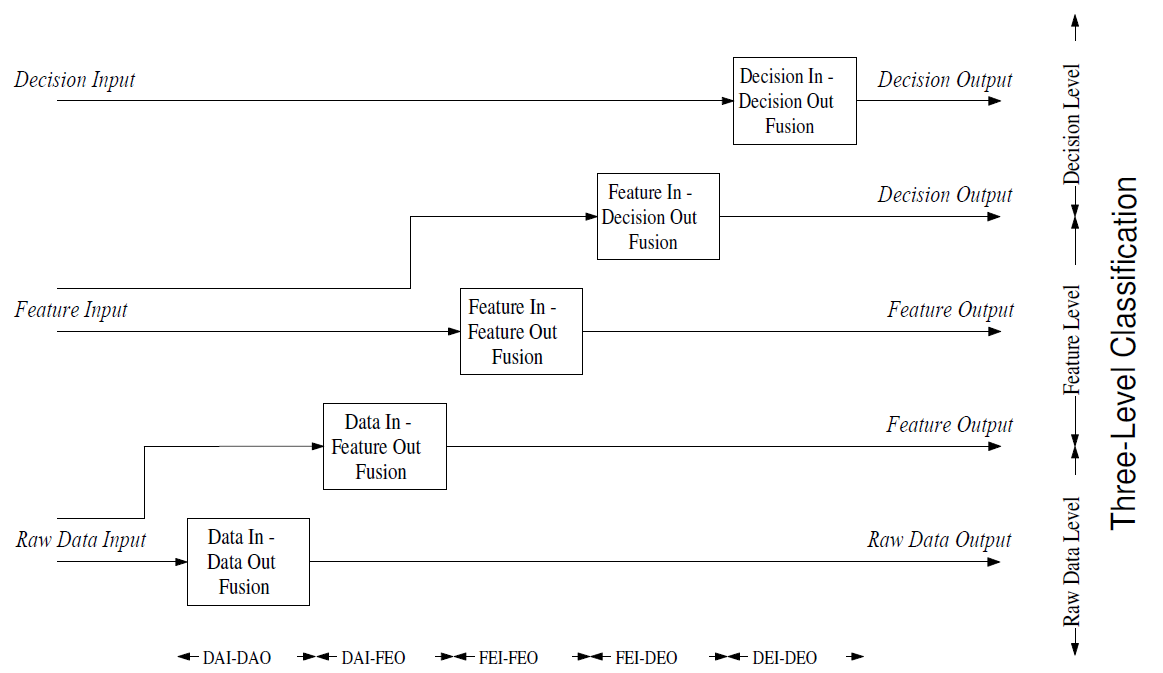
\includegraphics[width=1.1\textwidth]{src/pic/InputoutputCat.png}
  \caption{Fusion Categorization by input/output}
  \label{fig:InputoutputCat}
\end{figure}

\subsection{Categorization Based on Sensor Configuration}
Sensor fusion may be in different configuration types. According to various configuration, sensor fusion can be categorized into three sections\cite{Wilfried2002}:
\begin{description}
    \item[Complementary:] A configuration is considered as a complementary configuration when the sensors participating in sensor fusion are not directly dependent on each other, but it would be a case where inputs of the sensors are mixed to produce complete result. This configuration solves on of the common problem of single sensor system which is incompleteness of sensor data.
    \item[Competitive:] Competitive configuration can be achieved by keeping multiple sensors for observing same object or view which are independent from each other. This configuration ensure high redundancy of data and that is why it is also called \emph{redundant configuration}\cite{Wilfried2002}.
    \item[Cooperative:] A cooperative mechanism is the intelligent one in a sense that in this configuration the inputs from separate sensors are combined to produce a information which is not available in the single sensor inputs. An example for a cooperative sensor configuration is stereoscopic vision - by combining two-dimensional images from two cameras at slightly different viewpoints a three-dimensional image of the observed scene is derived\cite{Wilfried2002}.
\end{description}

There could be more categories exists but commonly used sensors are categorized like above. 

\section{Commonly used Sensor Fusion Models/Applications}

